\documentclass[aps,prd,twocolumn,superscriptaddress,nofootinbib,amsmath,amssymb,floatfix,10pt]{revtex4-2}

\usepackage{booktabs}
\usepackage{graphicx}
\usepackage{xurl}
\usepackage[hidelinks]{hyperref}
\graphicspath{{figures/}{paper_draft/workflow_architecture_v1/figures/}}

\hypersetup{
  pdftitle={A Content-Addressed Workflow for Reproducible DANTE Gravitational-Wave Anomaly Analysis},
  pdfauthor={Luca Cirfeta},
  pdfsubject={Architecture and verification of the DANTE local scientific workflow},
  pdfkeywords={gravitational waves, anomaly detection, reproducibility, provenance, scientific workflows}
}

\newcommand{\dante}{\textsc{Dante}}

\begin{document}

\title{\texorpdfstring{A Content-Addressed Workflow for Reproducible\\
DANTE Gravitational-Wave Anomaly Analysis}{A Content-Addressed Workflow for
Reproducible DANTE Gravitational-Wave Anomaly Analysis}}

\author{Luca Cirfeta}
\thanks{ORCID: \href{https://orcid.org/0009-0000-1235-3186}{0009-0000-1235-3186}}
\affiliation{Independent Researcher, Rome, Italy}
\date{Draft of \today}

\begin{abstract}
Unsupervised analysis of gravitational-wave detector data combines expensive
scientific stages with data acquisition, provenance checks, statistical
calibration, follow-up products, and reporting.  Reproducing such an analysis
requires more than preserving model weights or a final candidate table: the
execution graph, scientific contracts, retry semantics, and verification
boundary must also be explicit.  We present a local workflow layer for the
Domain-Adaptive Network for Transient Evaluation (\dante{}) that represents a
corrected O4a analysis as a content-addressed, 15-stage directed acyclic graph.
The architecture separates immutable stage evidence from mutable operational
progress, binds command-line and browser interfaces to the same run identity,
and resumes only work compatible with the frozen contract.  The tagged v1
release records all 15 stages as verified in a machine-readable receipt and
passed a documented human usability gate.  The release verifies adopted
scientific artifacts rather than recomputing them, and therefore makes no new
claim of global significance, astrophysical discovery, or public real-time
operation.  This paper describes the architecture, its fail-closed controls,
and the bounded evidence supporting reproducible local use.
\end{abstract}

\maketitle

\section{Introduction}
\label{sec:introduction}

Computational reproducibility in detector characterization depends on the
identity of data, code, configuration, execution environment, and intermediate
artifacts.  A scientifically correct stage can still be difficult to reproduce
when its ordering, retry behavior, or upstream evidence is implicit.  This work
addresses that operational layer for \dante{} without changing what the
underlying anomaly analysis measures or how its statistical decisions are
validated.

The contribution is a versioned workflow contract, a durable state model, a
shared command-line and local-web control path, and a final receipt that exposes
verified artifacts only after their stage gates pass.  The implementation is
frozen by an annotated release tag.  The corresponding machine-readable
receipt is distributed in the tagged source tree.

\section{Scope and threat model}
\label{sec:scope}

The workflow guards against accidental parameter drift, incompatible resume,
duplicate execution, partial evidence, interface-specific identities, and the
presentation of unverified outcomes.  It does not claim tolerance to arbitrary
hardware failure, distributed execution, hostile multi-user access, or
equivalence between CPU and CUDA environments.  It is a local single-user
controller, not an alerting service.

\section{Scientific and orchestration boundaries}
\label{sec:boundaries}

Scientific configuration and stage verifiers remain authoritative.  The
orchestration layer orders those stages, records their identities, and refuses
incompatible evidence; it does not duplicate scoring, threshold, bootstrap,
coincidence, or environmental-monitor logic.  The released workflow adopts and
re-verifies existing corrected-O4a artifacts.  It does not independently
recompute the scientific chain.

\section{Workflow architecture}
\label{sec:architecture}

The frozen graph contains 15 stages from preflight and acquisition through
calibration, scanning, native adaptation, follow-up, comparison, and reporting.
The native-calibration node depends both on the cohort and on the window
manifest consumed by the native index, preserving the frozen exclusion guard
before rescoring.  Figure~\ref{fig:dag} is generated directly from the
versioned workflow configuration; the layout is fixed for readability, while
the stage and dependency sets are validated against the contract at generation
time.

\begin{figure*}[t]
\centering
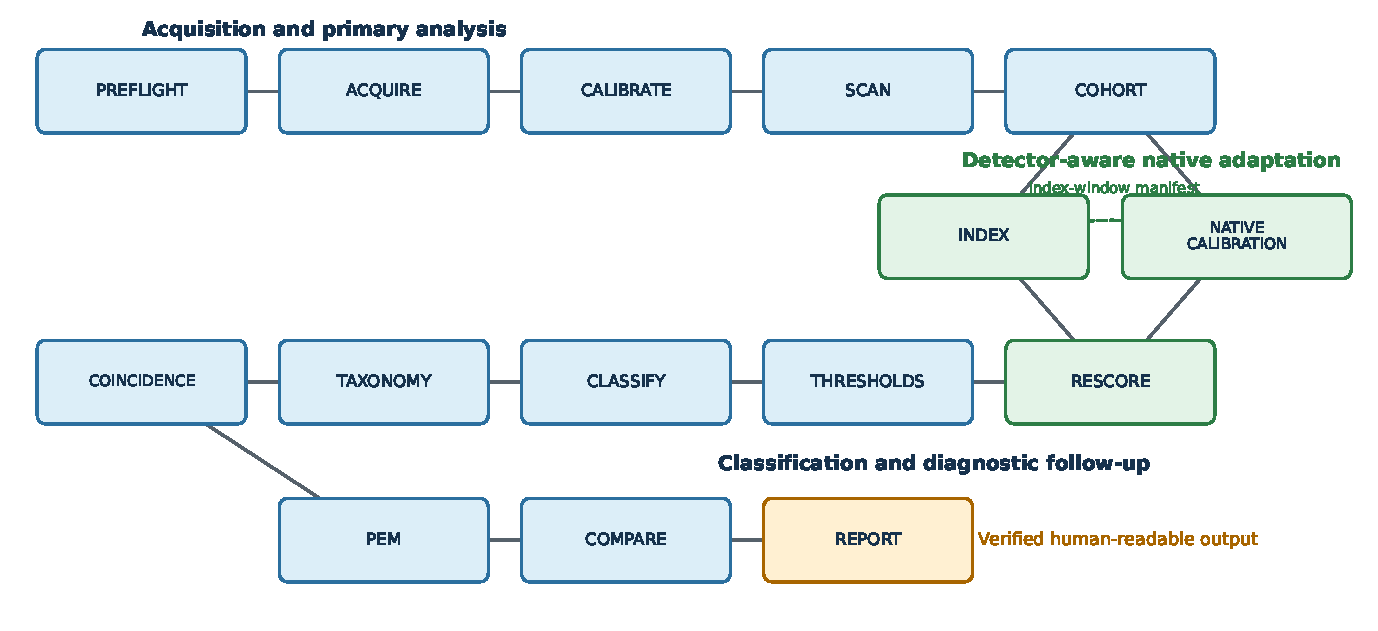
\includegraphics[width=\textwidth]{fig_workflow_dag.pdf}
\caption{The frozen 15-stage workflow.  Solid arrows are verified stage
dependencies.  The dashed green edge is the content-digested index-window
manifest consumed by native calibration; it makes the exclusion relationship
explicit before both native products enter rescoring.}
\label{fig:dag}
\end{figure*}

\section{Identity, state, and provenance}
\label{sec:provenance}

This section will specify run keys, attempt directories, leases, stage
receipts, artifact digests, and the final release receipt.  It will distinguish
mutable progress reporting from immutable scientific evidence and document the
conditions under which retry, reuse, or fail-closed rejection occurs.

\begin{figure*}[t]
\centering
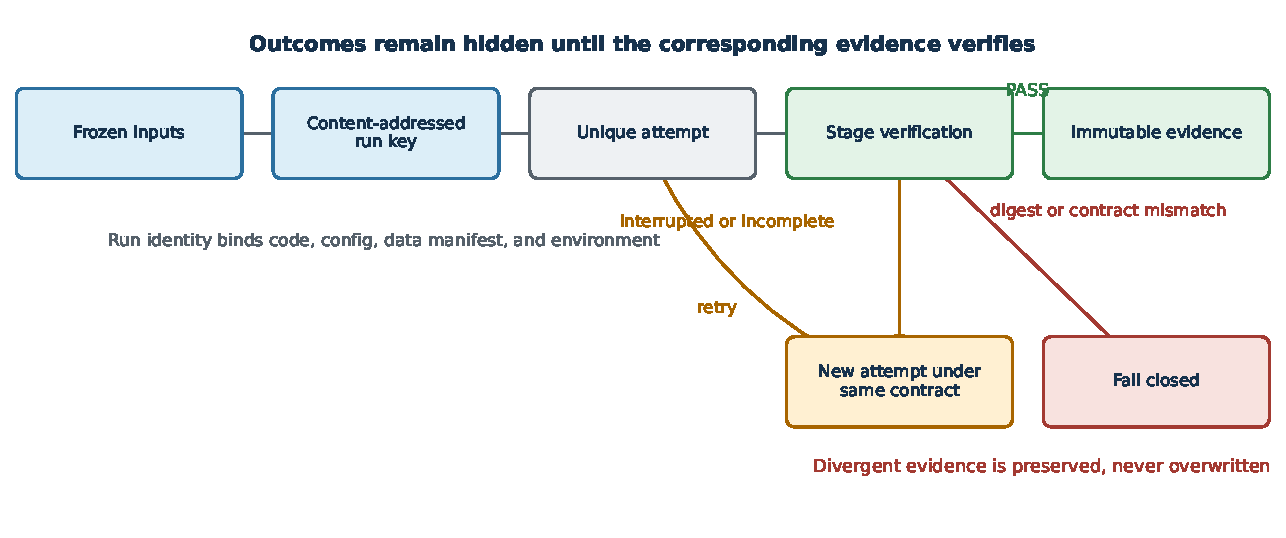
\includegraphics[width=0.96\textwidth]{fig_evidence_lifecycle.pdf}
\caption{Evidence lifecycle.  Incomplete work receives a new attempt under the
same contract, whereas a digest or contract mismatch fails closed.  Verified
evidence is immutable and outcome-bearing fields remain hidden until the
corresponding gate passes.}
\label{fig:evidence}
\end{figure*}

\section{Operator interfaces and recovery}
\label{sec:interfaces}

The command-line and browser interfaces invoke the same orchestrator.  The
browser is a loopback-only reader and controller; the workflow worker remains a
separate process.  The final draft will describe device guidance, progress and
ETA semantics, detailed logs, interruption recovery, and the dedicated
verification-results view.

\begin{figure*}[t]
\centering
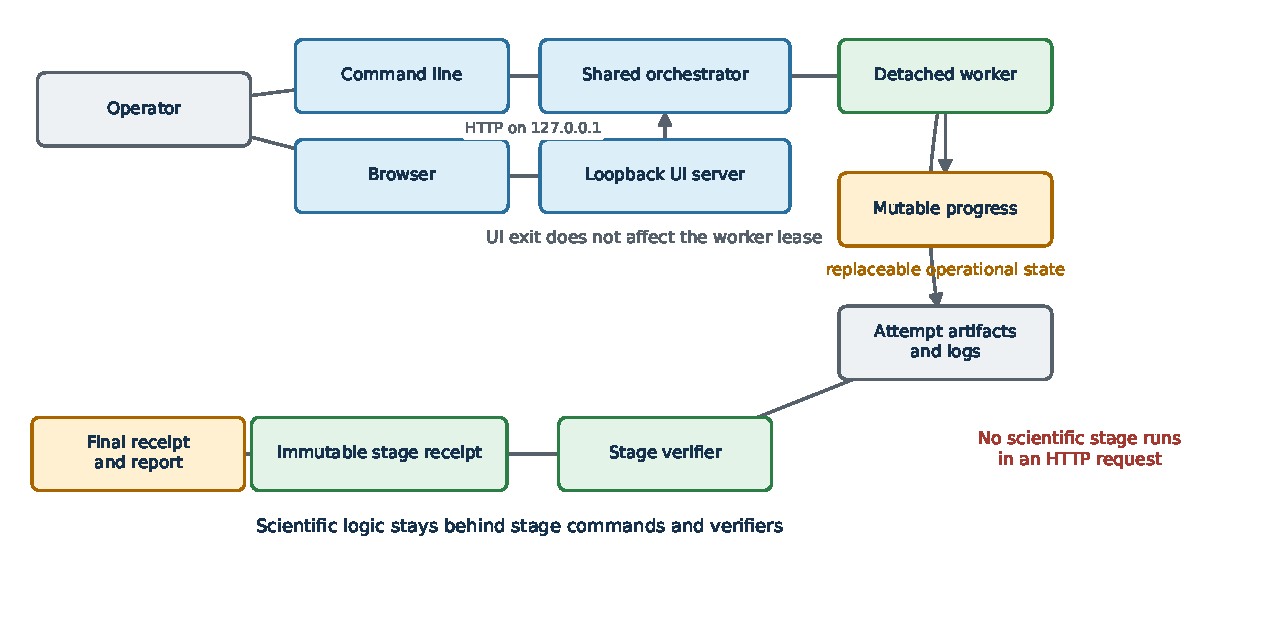
\includegraphics[width=0.96\textwidth]{fig_runtime_boundary.pdf}
\caption{Runtime boundary shared by the command-line and browser paths.  The
loopback UI is a disposable controller; the detached worker, durable attempts,
and stage verifiers remain authoritative.  Scientific stage logic is not
executed inside HTTP request handlers.}
\label{fig:runtime}
\end{figure*}

\section{Verification methodology}
\label{sec:verification}

Verification evidence includes schema and process tests, clean-clone public
smoke execution, command-line/browser identity parity, failure injection,
interruption recovery, final receipt verification, and human usability
acceptance.  Each test population and limitation will be reported separately;
technical smoke evidence will not be represented as a full scientific rerun.

\section{Results}
\label{sec:results}

The tagged release receipt reports \texttt{PASS\_VERIFIED\_WORKFLOW} for the
15-stage graph.  This section will present the exact release identities and the
bounded acceptance matrix directly from versioned evidence.  It will not
interpret candidate outcomes or convert engineering checks into statistical
significance.

\section{Limitations}
\label{sec:limitations}

The release is local and single-user, relies on pinned external scientific
artifacts, and distinguishes rather than equates CPU and CUDA identities.  Its
adopted-stage verification does not substitute for a new end-to-end O4a
recalculation.  Coincidence and environmental-monitor products remain
diagnostic follow-up evidence, and no global-significance or discovery claim
follows from workflow verification.

\section{Reproducibility}
\label{sec:reproducibility}

The public reproduction path, environment requirements, commands, expected
artifacts, and verification procedure will be transcribed from the tagged
quickstart and receipt.  The final arXiv bundle will include a source manifest
and cryptographic digests but no automated publication step.

\section{Conclusion}
\label{sec:conclusion}

The implemented workflow makes the operational contract of a complex anomaly
analysis explicit and machine-verifiable while preserving the authority and
limits of its scientific stages.  The remaining manuscript work is to present
the frozen architecture and its evidence completely, not to broaden the
scientific claims of the corrected O4a analysis.

\end{document}
